\documentclass[10pt]{article}
\usepackage[nu,tightmargin]{esial}
%\usepackage[nu,tightmargin,correction]{esial}
\TOP\1A

\usepackage[utf8x]{inputenc}
\usepackage{marvosym}
\usepackage{eurosym}
\usepackage{url}
\usepackage{amstext,amsmath,amsfonts}
\usepackage{fancyvrb}
\usepackage{graphicx}
%\usepackage[color,all]{xypic}
%\usepackage{xyling}
\usepackage{starsection}
\usepackage{tikz}
\usepackage{epsfig}

\hyphenpenalty=10000
\parindent0pt

\addtolength{\parskip}{.5em}

\renewcommand{\labelenumi}{(\alph{enumi})}
\newcommand{\Sedge}[1]{\Bk{-1.2}{1.2}{#1}}
\newcommand{\bareme}[1]{{\footnotesize (#1~pt)}}
\newcommand{\TODO}[1]{\emph{#1}\marginpar{\textsf{*ToDo*}}}

\newcommand{\BoxRep}{\ifcorrection{\boxtimes}{\Box}}
\newcommand{\boite}{$\Box$\xspace}
\newcommand{\boiteRep}{$\BoxRep$\xspace}

%\newcommand{\codebox}[1]{\fbox{\footnotesize\texttt{#1}\normalsize}}
%\newcommand{\codebox}[1]{\footnotesize\texttt{#1}\normalsize}
%\newcommand{\code}[1]{\footnotesize\texttt{#1}\normalsize}
\newcommand{\codebox}[1]{\texttt{#1}}
\newcommand{\code}[1]{\texttt{#1}}


\newcommand{\crccard}[3]{%
\begin{center}
\fbox{%
\begin{tabular}{p{115mm}|p{5cm}}
\multicolumn{2}{l}{\vspace{.2em} {\bf Classe : } #1 } \\
\hline
\vspace{.1em} {\bf Responsabilités : } & \vspace{.1em} {\bf Collaborateurs : }  \\
\vspace{-.5em}\raggedright #2 & \vspace{-.5em} #3 \\
\end{tabular}
}
\end{center}
}

\begin{document}
\color{black}
\title{Mini Projet 2008-2009}
\maketitle


\section*{Modalités}

Ce projet est à réaliser en binôme. Vous indiquerez la composition de
votre binôme dans un fichier dénommé \texttt{AUTHORS} (placé  à la
racine du répertoire de votre projet) qui doit contenir les logins
UNIX des membres du groupe, un par ligne.


{\bf Travail à rendre :} Vous devez rendre un mini-rapport de projet (5 pages
maximum, format pdf) en plus de vos fichiers sources.  Vous y détaillerez les
difficultés auxquelles vous avez été confronté, et comment vous les avez
résolues. Vous indiquerez également le nombre d'heures passées sur les
différentes étapes de ce projet (conception, codage, tests, rédaction du
rapport) par chaque membre du groupe.

{\bf Comment rendre votre projet :} Vous devez placer les fichiers nécessaires
dans un répertoire sur neptune, vous placer dedans, et invoquer la commande
suivante (seuls les fichiers sources (et le pdf) sont copiés). Vous pouvez
lancer le script autant de fois que vous le souhaitez, seule la dernière
soumission est conservée.
\begin{center}
\fbox{\texttt{/home/EqPedag/quinson/bin/rendre\_projet TOP}}

{\Large Avant le 21 Mars 2009, à 23h59.} 

(le script n'acceptera pas de soumission en retard)
\end{center}

Un projet ne compilant pas sera sanctionnée par une note adéquate. Toute
soumission par email sera refusée.

{\bf Évaluation :} Des soutenances individuelles de projet seront organisées la
semaine du \underline{22 Mars 2009}. Vous serez jugé sur la qualité de votre
programme, celle de votre rapport et votre capacité à expliquer son
fonctionnement. Vous aurez également à répondre à des questions en rapport avec
les TP effectués dans le module, sans rapport  avec le projet.

\section*{Travail personnel et honnêteté}

\begin{quote}
Ne trichez pas! Ne copiez pas!
Si vous le faites, vous serez lourdement sanctionnés. Nous ne ferons pas de distinction entre copieur et copié.
Vous n'avez pas de (bonne) raison de copier. En cas de problème, nous sommes prêt à vous aider. 
Encore une fois: en cas de doute, envoyez un courriel à vos enseignants, ça ne les dérange pas.

Par tricher, nous entendons notamment :
\begin{itemize}
  \item Rendre le travail d'un collègue avec votre nom dessus ;
  \item Obtenir une réponse par Google\texttrademark{} ou autre et mettre votre nom dessus ;
  \item Récupérer du code et ne changer que les noms de variables et fonctions ou leur ordre avant de mettre votre nom dessus
      (\emph{``moving chunks of code around is like moving food around on your plate to diguise the fact that you havn't eated all your brussel sprouts''}) ;
  \item Permettre à un collègue de \emph{s'inspirer} de votre travail. Assurez vous que votre répertoire de travail n'est lisible que par vous même.
\end{itemize}

Il est plus que très probable que nous détections les tricheries. Chacun a son propre style de programmation, et personne ne code la même chose de la même manière. De plus, il existe des programmes très efficaces pour détecter les similarités douteuses entre copies (MOSS, \url{http://theory.stanford.edu/~aiken/moss/}).

\medskip
En revanche, il est possible (voire conseillé) de discuter du projet et
d'échanger des idées avec vos collègues. Mais vous ne pouvez rendre que du code
écrit par vous-même. Vous indiquerez dans votre rapport toutes vos sources
d'inspiration (comme les sites internet de vulgarisation de l'informatique que
vous auriez consulté).

\end{quote}


\section*{Bibliographie}

Le problème présenté a été proposé par Stephen Weiss en 2003 en tant que \emph{Nifty Assignment} au groupe 
d'intérêt \emph{ACM Special Interest Group on Computer Science Education (SIGCSE)}. Le sujet original peut être consulté à l'adresse suivante : \url{http://nifty.stanford.edu/2003/backtracking/}.

La documentation de l'API Java : \url{http://java.sun.com/javase/6/docs/api/}.

Vous pourrez trouver des informations complémentaires à l'adresse suivante:\\
\url{http://www.loria.fr/~quinson/teach-prog.html#faqTOP}

\clearpage
\section*{Présentation du problème : 9-square puzzle}


Imprimer cette page et découper les neuf carrés. Ensuite, essayer d'arranger ces carrés en une grille $3 \times 3$ tels que pour deux carrés adjacents la somme des valeurs côte-à-côte soit égale à 0. Bien entendu vous êtes autorisés à faire pivoter les carrés.

\begin{center}
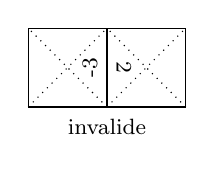
\begin{tikzpicture}[scale=1]
    \draw (0,1) -- (1,1) ; \draw (0.5,1) ;
    \draw (1,1) -- (1,0) ; \draw (1,0.5) node[above,rotate=90] {\footnotesize -3} ;
    \draw (1,0) -- (0,0) ; \draw (0.5,0) ;
    \draw (0,0) -- (0,1) ; \draw (0,0.5) ;
    \draw[dotted] (0,0) -- (1,1) ; \draw[dotted] (1,0) -- (0,1) ;

    \draw (1,1) -- (2,1) ; \draw (1.5,1) ;
    \draw (2,1) -- (2,0) ; \draw (2,0.5) ;
    \draw (2,0) -- (1,0) ; \draw (1.5,0) ;
    \draw (1,0) -- (1,1) ; \draw (1,0.5) node[above,rotate=270] {\footnotesize 2} ;
    \draw[dotted] (1,0) -- (2,1) ; \draw[dotted] (2,0) -- (1,1) ; 
    
    \draw (1, -0.25) node {\footnotesize invalide};
\end{tikzpicture}
\hspace{2cm}
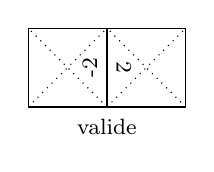
\begin{tikzpicture}[scale=1]
    \draw (0,1) -- (1,1) ; \draw (0.5,1) ;
    \draw (1,1) -- (1,0) ; \draw (1,0.5) node[above,rotate=90] {\footnotesize -2} ;
    \draw (1,0) -- (0,0) ; \draw (0.5,0) ;
    \draw (0,0) -- (0,1) ; \draw (0,0.5) ;
    \draw[dotted] (0,0) -- (1,1) ; \draw[dotted] (1,0) -- (0,1) ;

    \draw (1,1) -- (2,1) ; \draw (1.5,1) ;
    \draw (2,1) -- (2,0) ; \draw (2,0.5) ;
    \draw (2,0) -- (1,0) ; \draw (1.5,0) ;
    \draw (1,0) -- (1,1) ; \draw (1,0.5) node[above,rotate=270] {\footnotesize 2} ;
    \draw[dotted] (1,0) -- (2,1) ; \draw[dotted] (2,0) -- (1,1) ; 
    
    \draw (1, -0.25) node {\footnotesize valide};
\end{tikzpicture}
\end{center}

Sachez qu'il y a $4^9 \times 9! =  95~126~814~720$ arrangements possibles, et que l'instance du problème donnée ci-dessous n'admet que 4 solutions (en réalité 4 rotations de la même solution). 


\begin{center}
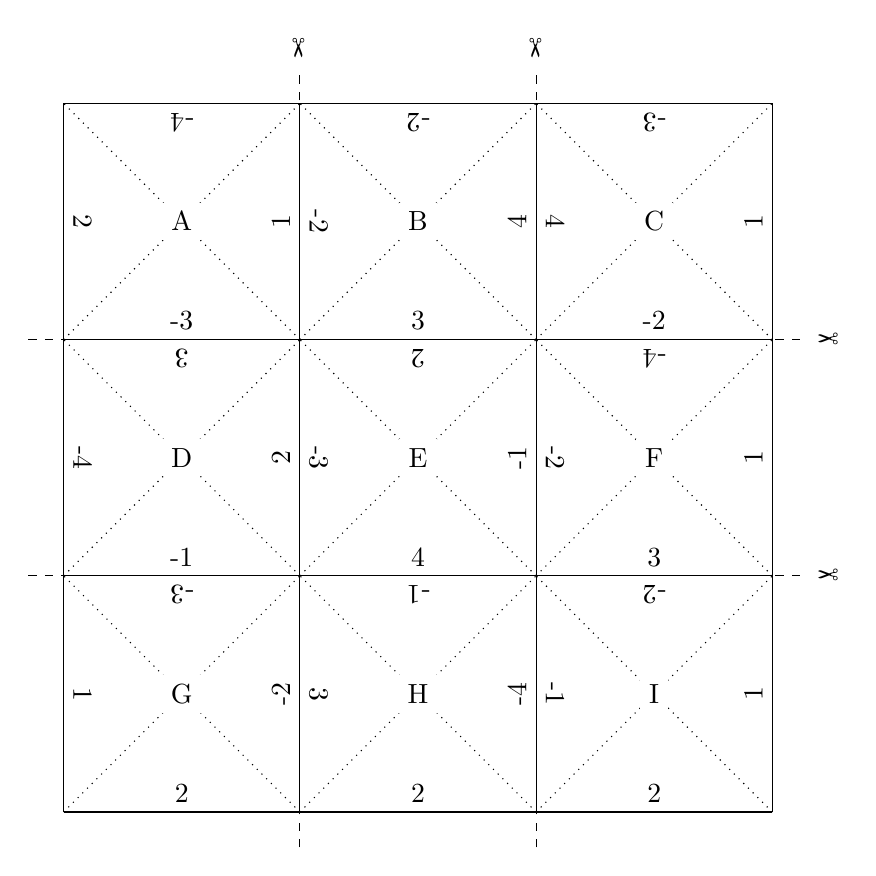
\begin{tikzpicture}[scale=3]

    \draw (0,3) -- (1,3) ; \draw (0.5,3) node[above,rotate=180]   {-4} ; % top
    \draw (1,3) -- (1,2) ; \draw (1,2.5) node[above,rotate=90]    {1}  ; % right
    \draw (1,2) -- (0,2) ; \draw (0.5,2) node[above]              {-3} ; % bottom
    \draw (0,2) -- (0,3) ; \draw (0,2.5) node[above,rotate=270]   {2}  ; % left
    \draw[dotted] (0,2) -- (1,3) ; \draw[dotted] (1,2) -- (0,3) ; % diag 
    \draw (0.5,2.5) node[fill=white] {A} ;

    \draw (1,3) -- (2,3) ; \draw (1.5,3) node[above,rotate=180]   {-2} ; % top
    \draw (2,3) -- (2,2) ; \draw (2,2.5) node[above,rotate=90]    {4}  ; % right
    \draw (2,2) -- (1,2) ; \draw (1.5,2) node[above]              {3}  ; % bottom
    \draw (1,2) -- (1,3) ; \draw (1,2.5) node[above,rotate=270]   {-2} ; % left
    \draw[dotted] (1,2) -- (2,3) ; \draw[dotted] (2,2) -- (1,3) ; % diag 
    \draw (1.5,2.5) node[fill=white] {B} ;

    \draw (2,3) -- (3,3) ; \draw (2.5,3) node[above,rotate=180]   {-3} ; % top
    \draw (3,3) -- (3,2) ; \draw (3,2.5) node[above,rotate=90]    {1}  ; % right
    \draw (3,2) -- (2,2) ; \draw (2.5,2) node[above]              {-2} ; % bottom
    \draw (2,2) -- (2,3) ; \draw (2,2.5) node[above,rotate=270]   {4}  ; % left
    \draw[dotted] (2,2) -- (3,3) ; \draw[dotted] (3,2) -- (2,3) ; % diag 
    \draw (2.5,2.5) node[fill=white] {C} ;

    \draw (0,2) -- (1,2) ; \draw (0.5,2) node[above,rotate=180]   {3}  ; % top
    \draw (1,2) -- (1,1) ; \draw (1,1.5) node[above,rotate=90]    {2}  ; % right
    \draw (1,1) -- (0,1) ; \draw (0.5,1) node[above]              {-1} ; % bottom
    \draw (0,1) -- (0,2) ; \draw (0,1.5) node[above,rotate=270]   {-4} ; % left
    \draw[dotted] (0,1) -- (1,2) ; \draw[dotted] (1,1) -- (0,2) ; % diag 
    \draw (0.5,1.5) node[fill=white] {D} ;

    \draw (1,2) -- (2,2) ; \draw (1.5,2) node[above,rotate=180]   {2}  ; % top
    \draw (2,2) -- (2,1) ; \draw (2,1.5) node[above,rotate=90]    {-1} ; % right
    \draw (2,1) -- (1,1) ; \draw (1.5,1) node[above]              {4}  ; % bottom
    \draw (1,1) -- (1,2) ; \draw (1,1.5) node[above,rotate=270]   {-3} ; % left
    \draw[dotted] (1,1) -- (2,2) ; \draw[dotted] (2,1) -- (1,2) ; % diag 
    \draw (1.5,1.5) node[fill=white] {E} ;

    \draw (2,2) -- (3,2) ; \draw (2.5,2) node[above,rotate=180]   {-4} ; % top
    \draw (3,2) -- (3,1) ; \draw (3,1.5) node[above,rotate=90]    {1}  ; % right
    \draw (3,1) -- (2,1) ; \draw (2.5,1) node[above]              {3}  ; % bottom
    \draw (2,1) -- (2,2) ; \draw (2,1.5) node[above,rotate=270]   {-2} ; % left
    \draw[dotted] (2,1) -- (3,2) ; \draw[dotted] (3,1) -- (2,2) ; % diag 
    \draw (2.5,1.5) node[fill=white] {F} ;

    \draw (0,1) -- (1,1) ; \draw (0.5,1) node[above,rotate=180]   {-3} ; % top
    \draw (1,1) -- (1,0) ; \draw (1,0.5) node[above,rotate=90]    {-2} ; % right
    \draw (1,0) -- (0,0) ; \draw (0.5,0) node[above]              {2}  ; % bottom
    \draw (0,0) -- (0,1) ; \draw (0,0.5) node[above,rotate=270]   {1}  ; % left
    \draw[dotted] (0,0) -- (1,1) ; \draw[dotted] (1,0) -- (0,1) ; % diag 
    \draw (0.5,0.5) node[fill=white] {G} ;

    \draw (1,1) -- (2,1) ; \draw (1.5,1) node[above,rotate=180]   {-1} ; % top
    \draw (2,1) -- (2,0) ; \draw (2,0.5) node[above,rotate=90]    {-4} ; % right
    \draw (2,0) -- (1,0) ; \draw (1.5,0) node[above]              {2}  ; % bottom
    \draw (1,0) -- (1,1) ; \draw (1,0.5) node[above,rotate=270]   {3}  ; % left
    \draw[dotted] (1,0) -- (2,1) ; \draw[dotted] (2,0) -- (1,1) ; % diag 
    \draw (1.5,0.5) node[fill=white] {H} ;

    \draw (2,1) -- (3,1) ; \draw (2.5,1) node[above,rotate=180]   {-2} ; % top
    \draw (3,1) -- (3,0) ; \draw (3,0.5) node[above,rotate=90]    {1}  ; % right
    \draw (3,0) -- (2,0) ; \draw (2.5,0) node[above]              {2}  ; % bottom
    \draw (2,0) -- (2,1) ; \draw (2,0.5) node[above,rotate=270]   {-1} ; % left
    \draw[dotted] (2,0) -- (3,1) ; \draw[dotted] (3,0) -- (2,1) ; % diag 
    \draw (2.5,0.5) node[fill=white] {I} ;

    \draw[dashed] (1,-0.15) --(1,3.15) node[right,rotate=90] {\Leftscissors}; 
    \draw[dashed] (2,-0.15) --(2,3.15) node[right,rotate=90] {\Leftscissors}; 
    \draw[dashed] (-0.15,1) --(3.15,1) node[right] {\Leftscissors}; 
    \draw[dashed] (-0.15,2) --(3.15,2) node[right] {\Leftscissors}; 

\end{tikzpicture}
\end{center}

{\bf Remarque :} Un puzzle est dit \emph{parfait} si chaque pièce contient une et une seule fois les nombres 1, 2, 3 et 4 dont deux sont positifs et deux sont négatifs. Le puzzle donné en exemple n'est donc pas parfait.

\section*{Travail à réaliser}

L'objectif de ce mini-projet de réaliser un programme reposant sur un algorithme récursif avec retour arrière (\emph{backtracking}) qui calcule les solutions à une instance du problème présenté précédemment.

Votre programme devra indiquer le nom du puzzle, si ce puzzle est parfait ou non. Il devra afficher le nombre de solutions trouvées ainsi que le détail de ces solutions. Il devra également afficher le temps de calcul total et d'autres statistiques que vous jugerez intéressantes (nombre d'appels récursifs, nombre de solutions explorées ou rejetées, \ldots).

Votre programme devra être capable de lire un fichier contenant la description de l'instance du problème à résoudre. Ce fichier respectera le format suivant : \\

~~~
\begin{minipage}{.3\linewidth}
  \VerbatimInput[label=data/data1.txt]{data/data1.txt}
\end{minipage}
~~~~
\begin{minipage}{.5\linewidth}
  \begin{itemize}
     \item[$\bullet$] La première ligne contient un titre,
     \item[$\bullet$] les neuf lignes suivantes représentent chacune une pièce.
     \begin{itemize}
	   \item Une étiquette (un caractère),
	   \item les 4 valeurs de la pièce classées dans l'ordre des aiguilles d'une montre en commençant par la valeur du haut de la pièce.  
	 \end{itemize}
  \end{itemize}
\vfill
\end{minipage}


Vous trouverez sur \texttt{neptune} (\verb+/home/depot/1A/TOP/projets/data/+), différents fichiers contenant les différentes instances du problème que votre programme doit être capable de résoudre.


\section*{Bonus (tâches facultatives)}

\begin{itemize}
	\item Généraliser votre programme pour résoudre des problèmes dont la taille du plateau est variable et non plus seulement limitée à $3 \times 3$ pièces.
	\item Généraliser votre programme pour résoudre ce problème avec des pièces en forme de cube et non plus des pièces carrées.
\end{itemize}


\section*{Indications}

Dans ce projet vous devez mettre en applications les connaissances que vous avez acquises dans le module POO ainsi que dans le module TOP. 

Vous devrez donc réaliser un programme en respectant les principes de
la programmation objet. Il vous est donc fortement conseillé de
chercher à modéliser le problème en manipulant des classes et des
objets. Par exemple, vous serez amenés à définir une classe pour le
programme principal, une pour une pièce, une pour le plateau de jeu
(qui peut représenter soit une solution trouvée, soit une solution en cours de construction), 
une pour représenter le pot des pièces non placées, \ldots

Afin de vous aider, vous trouverez ci-dessous une proposition de description sous forme de classes du programme. Vous êtes libres d'en proposer/utiliser une autre.

\section*{Classe/Responsabilités/Collaborations}

\crccard{\code{puzzle.Piece}}{
  \begin{itemize}
    \item Conserve les 4 valeurs et l'étiquette d'une pièce carrée du puzzle.
	\item Gère l'affichage d'une pièce.
	\item Gère les rotations d'une pièce.
	\item Détermine si une pièce est \emph{parfaite} ou non.
  \end{itemize}
}{
}

\crccard{\code{puzzle.Pool}}{
  \begin{itemize}
    \item Conserve toutes les pièces d'un puzzle.
	\item Gère la disponibilité des pièces (une pièce ne peut être utilisée qu'une seule fois dans un plateau).
	\item Gère le chargement d'une liste de pièces depuis une sous-partie d'un fichier formaté.
	\item Détermine si l'ensemble des pièces est \emph{parfait} ou non.
  \end{itemize}
}{
  \begin{itemize}
    \item \code{puzzle.Piece}	
  \end{itemize}
}

\crccard{\code{puzzle.Board}}{
  \begin{itemize}
    \item Gère le placement d'une pièce sur un plateau tout en respectant les règles du puzzle.
    \item Gère l'affichage d'un plateau.	
  \end{itemize}
}{
  \begin{itemize}
    \item \code{puzzle.Piece}	
  \end{itemize}
}

\crccard{\code{puzzle.NineSquarePuzzle}}{
  \begin{itemize}
    \item Détermine si une instance du puzzle est \emph{parfaite} ou non.
	\item Résout une instance du puzzle.
	\item Conserve les solutions trouvées.
	\item Gère le chargement d'un instance d'un puzzle à partir d'un fichier formaté.
  \end{itemize}
}{
  \begin{itemize}
    \item \code{puzzle.Pool}
	\item \code{puzzle.Board}
	\item \code{puzzle.Piece}
  \end{itemize}
}

\crccard{\code{puzzle.Main}}{
  \begin{itemize}
    \item Interagit avec l'utilisateur (affichage, demande de saisie du fichier de données à charger, affichage des statistiques, \ldots).
    \item Crée une instance du problème (\code{NineSquarePuzzle}) et demande la résolution de cette instance.
  \end{itemize}
}{
  \begin{itemize}
    \item \code{puzzle.NineSquarePuzzle}
    \item \code{puzzle.Instrumentations}
  \end{itemize}
}

\crccard{\code{puzzle.Instrumentations}}{
  \begin{itemize}
    \item Collecte les différentes statistiques (temps d'exécution, nombre d'appels de méthode, \ldots).
    \item Gère l'affichage des statistiques collectées.
  \end{itemize}
}{
}

\'Etant donné que le nombre d'arrangements possibles est très élevé
($>$ 95 milliards de possibilités), il est important de bien mettre en
\oe uvre le \emph{backtracking} et surtout de limiter au maximum la recherche aux solutions potentielles (élaguer au plus tôt les branches menant des instances non valides).


% \section*{Critères d'évaluations}

% La notation tiendra compte : 
% \begin{itemize}
%   \item	de la clarté du code rendu et de la documentation (commentaires, procédure d'utilisation, \ldots) ;
%   \item	du choix approprié (ou non) des classes et des méthodes implémentées ;
%   \item	de la correction et de l'efficacité de votre programme. Un programme qui résout correctement toutes les instances du problème et qui effectue moins d'appels sera mieux considéré qu'un programme nécessitant beaucoup plus d'appels pour trouver le même nombre de solutions.
% \end{itemize}

\newpage
\section*{Cas d'utilisation}

Vous trouverez ci-dessous à titre d'exemple, l'affichage donné lors l'utilisation du programme que vous devez réaliser.

\VerbatimInput[label=...,numbers=none,fontsize=\footnotesize]{output-small.txt}   





\end{document}
